\chapter{Fundamentação Teórica}
\label{chap:teoria}

Neste capítulo serão apresentados as bases teóricas levantadas para este trabalho.
O fluxo de conteúdo está organizado de forma a delimitar o domínio de atuação
do trabalho, partindo da visão macro, DevOps, até a visão micro, ferramentas de
extração de configuração, que é o foco deste trabalho. As seções estão dispóstas em:

\begin{itemize}
  \item \textbf{DevOps}: as definições e conceitos relacionados a DevOps;
  \item \textbf{Métodos Ágeis e DevOps}: conceitos de métodos ágeits e as suas relações com DevOps;
  \item \textbf{Automação}: o conceito de automação dentro da cultura DevOps e as suas vantagens;
  \item \textbf{Extração de Configuração}: formas de extração das configurações de ambiente;
\end{itemize}

\section{DevOps}
\label{sec:devops}

O termo DevOps tem sido usado com frequência em diversas esferas do
desenvolvimento de software da atualidade, mas por ser um conceito recente
(2008), muita cunfusão ainda é gerada ao tentar definir e trabalhar com
DevOps~\cite{adambertram:2016}. A palavra DevOps vem de duas palavras em
inglês, \textit{development} e \textit{operations} (desenvolvimento e operações) e de maneira
geral é a cultura, movimento ou conjunto de práticas que incentiva
a comunicação, a colaboração e a integração de desenvolvedores de software
e outros profissionais de TI. Além das práticas também engloba ferramentas
e técnicas que automatizam o processo de entrega de software e as mudanças
de infraestrutura~\cite{loukides2012devops}~\cite{erich2014mapping}.

Muitas vezes o termo é confundido com uma nova responsabilidade, ou cargo
dentro de uma empresa que desenvolve software, e por mais que seja possível
ter profissionais que tenham proficiência nas ferramentas relacionadas a
DevOps, o ideal, como dito anteriormente, é ter uma melhor comunicação,
colaboração e integração entre os times já existentes. As ferramentas
relacionadas à DevOps facilitam esses aspectos, mas o diferencial é a
mudança no processo de desenvolvimento para absorver essas melhorias
~\cite{adambertram:2016}.

%TODO: parece está faltando mais alguma coisa de DevOps

\section{Métodos Ágeis e DevOps}
\label{sec:agile-devops}

A metodologia Ágil surgiu como uma resposta às maneiras tradicionais de desenvolvimento
de software considerando uma nova abordagem com relação as práticas, organização,
documentação e foco no desenvolvimento.~\cite{agilemetorg:2016}

Os métodos ágeis são formas de sustentação da filosofia Ágil proposta no manifesto
Ágil\cite{fowler:2001}. As duas mais populares são o \textit{Scrum} e o \textit{Extreme Programming}. Nelas,
são definidas práticas que eram comumente utilizadas em outros contextos,
mas foram reunidas e adaptadas para se adequarem à filosofia Ágil~\cite{shore:2007}.

Diferentemente da metodologia de Cascata, por exemplo, o \textit{Scrum} implementa uma
abordagem iterativa e incremental, podendo assim desenvolver incrementos de
maior valor para o cliente mais cedo, e assim tendo \textit{feedback} para correções
mais frequentes. A Figura~\ref{fig:iterativ} mostra um exemplo dessas
Iterações.~\cite{scrumreference:2016}

\begin{figure}[H]
  \centering
  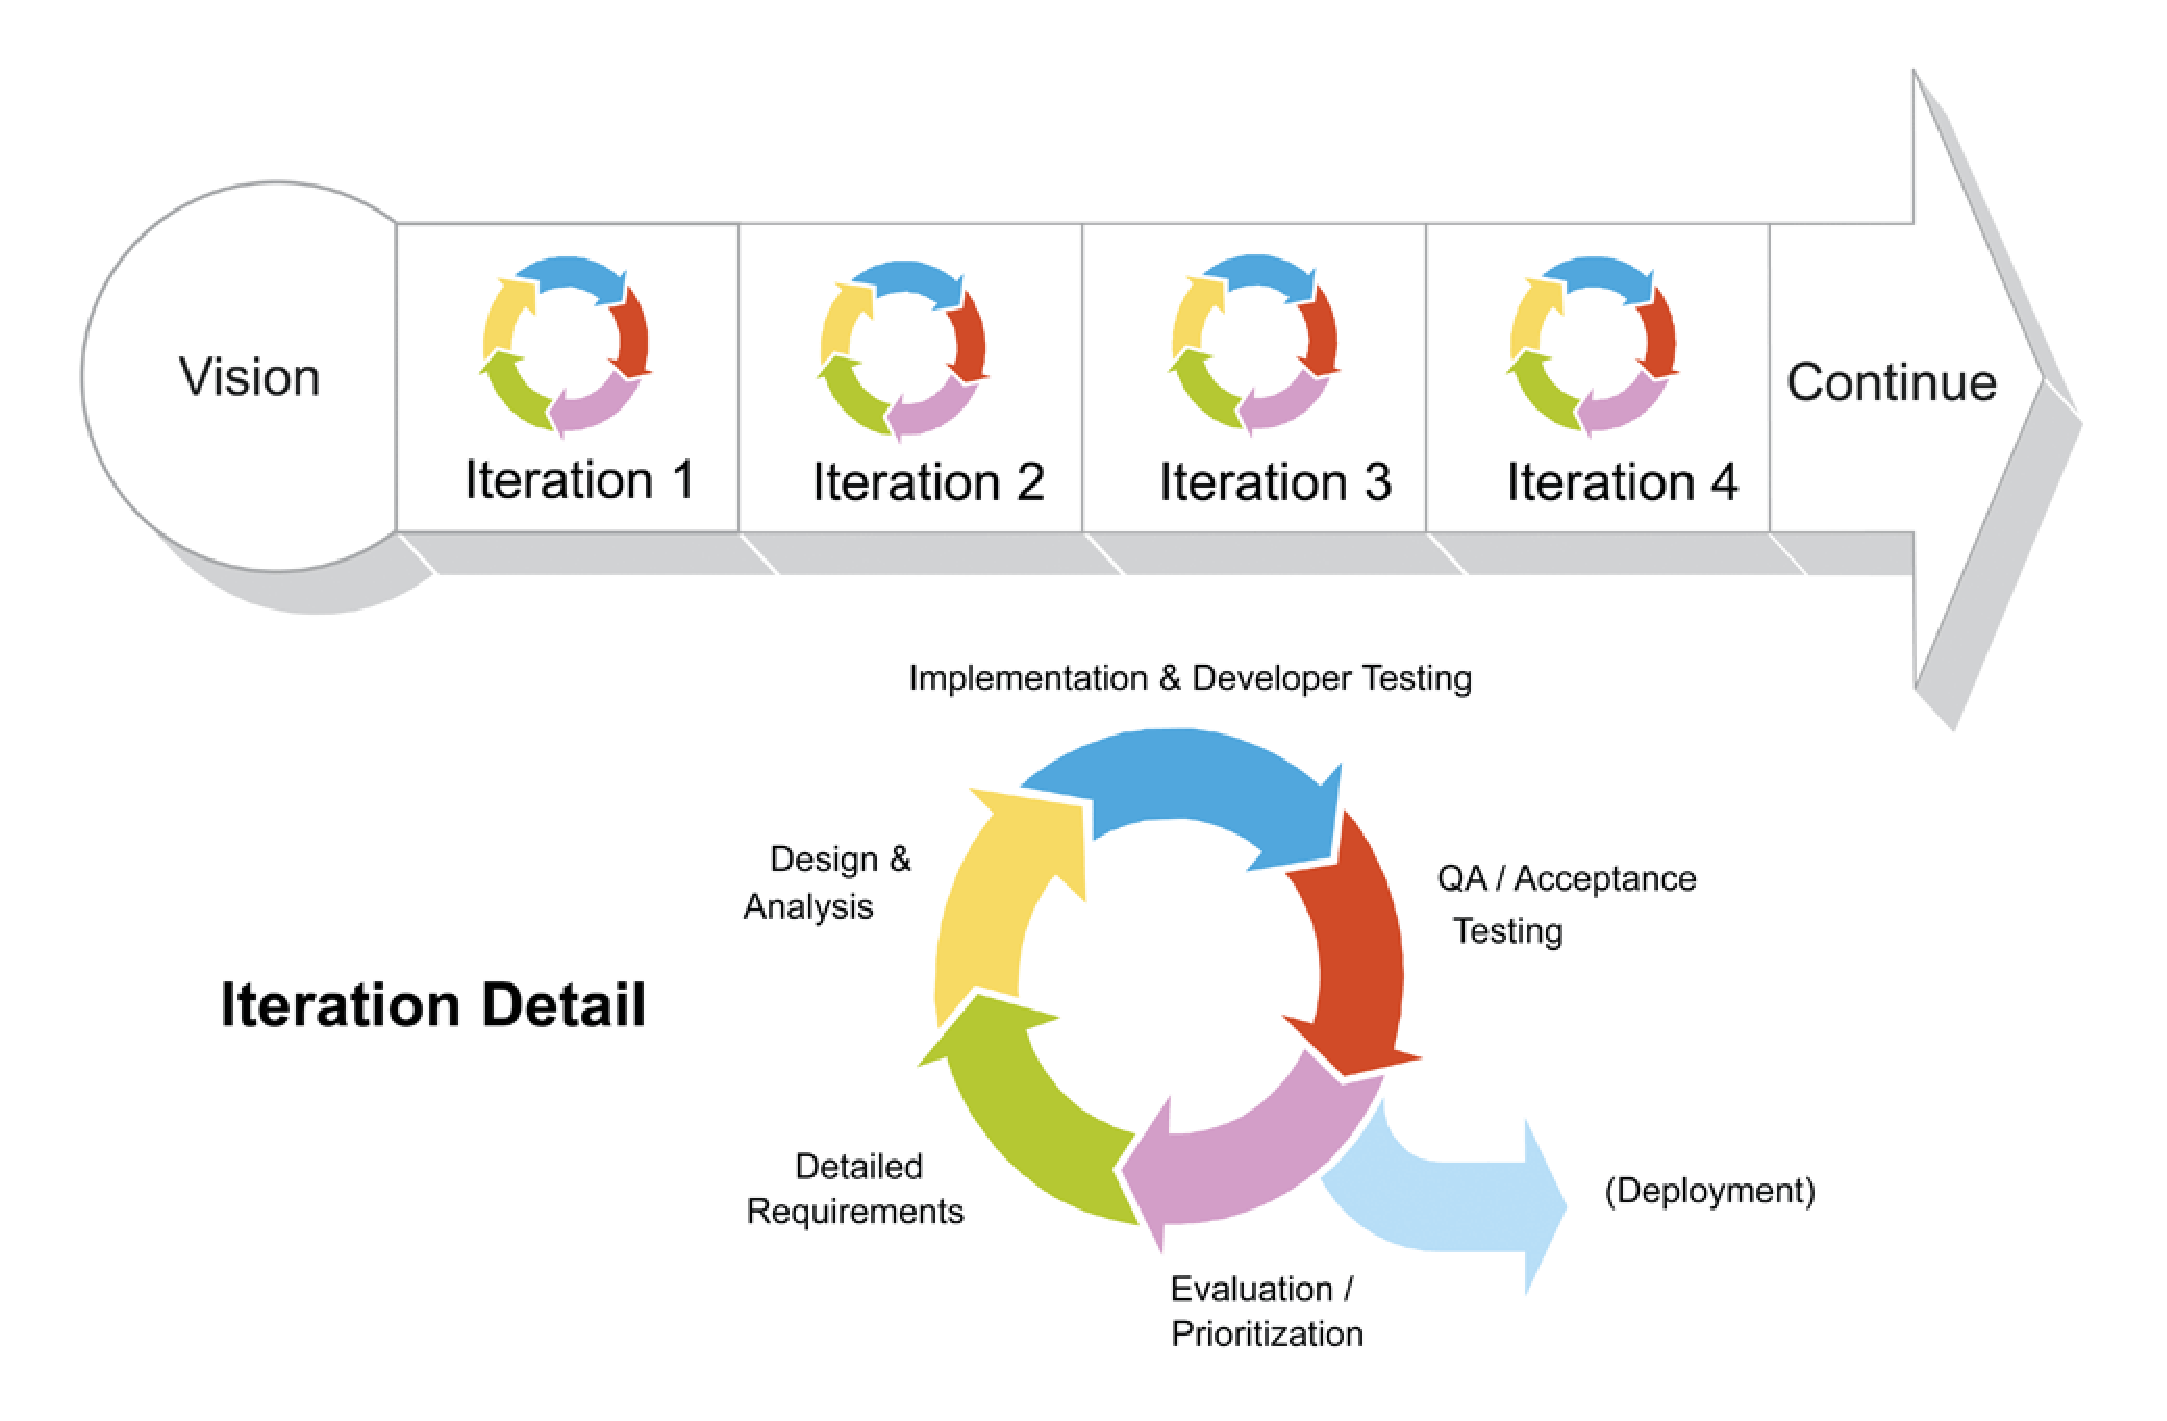
\includegraphics[width=0.8\textwidth]{figuras/iterative.eps}
  \caption{Iterações do Scrum~\cite{scrumreference:2016}.}
  \label{fig:iterativ}
\end{figure}

Com a popularização da metodologia de desenvolvimento Ágil, que tem, dentre outros
objetivos, o de entregar com maior frequência, e melhorar a comunicação entre os
times, é simples fazer a relação de DevOps com esse tipo de desenvolvimento.
DevOps nada mais é do que a implementação de conceitos e mudanças organizacionais
e culturais provenientes do pensamento Ágil~\cite{scott2014}.

DevOps tenta alcançar entregas mais frequentes ao preparar um ambiente que facilite,
automatize e integre vários dos processos que antes seriam manuais, e mais
suscetíveis à falhas e atrasos, o que não é possível sem uma equipe integrada
nesse ambiente. Dessa forma, o conceito de entrega contínua e de integração
contínua estão fortemente relacionados à DevOps.~\cite{adambertram:2016}

\subsection{Integração Contínua}

Integração contínua é a prática de integrar diversas partes de um software
desenvolvido em diversas frentes, de maneira periódica, ou a cada mudança.
Foi adotado como parte do método \textit{Extreme Programming} (XP) que sugere integrar
partes do software mais de uma vez por dia \cite{fowler2006continuous}.

Mesmo que não se adote desenvolvimento orientado a teste 
(TDD - \textit{test driven development}), uma funcionalidade só está 
pronta se estiver com seus testes implementados, levando em consideração 
metodologias de desenvolvimento Ágil. E, dessa forma, a integração 
contínua pode dar retorno com relação aos resultados desses testes a todo momento que ocorrer uma nova integração do software. %TODO: referencia

\subsection{Entrega Contínua}

A Entrega Contínua é uma prática adotada pelos métodos ágeis que tem o objetivo
de preparar um \textit{software} para que ele seja passível de ser posto em produção a
qualquer momento~\cite{olausson:2016}. 

A prática de Entrega Contínua  é frequentemente confundida com a Integração
Contínua. Existe uma relação de dependência entre as duas práticas para
construir uma estrutura que possa sustentar a entrega contínua de um
\textit{software}.~\citeonline{olausson:2016} resumem os dois em:

\begin{itemize}
  \item \textbf{Integração Contínua}: é voltada para estabelecer uma rápida
    validação da fase de desenvolvimento;
  \item \textbf{Entrega Contínua}: é voltada para estabelecer uma cultura onde
    pode-se oferecer um recurso ou \textit{feature} para o cliente a qualquer
    momento.
\end{itemize}


\section{Automação}
\label{sec:auto}

Em DevOps, a automação é um elemento essencial para se alcançar a maturidade
de entregas e \textit{feedback} rápidos. A automação consiste na execução
automática de um processo com o mínimo de intervensão humana. Para a área
de TI, a automação ocorre nos processos de controle e administração de
sistemas ou softwares~\cite{sharma:2015}.

Pode-se citar algumas das vantagens da automação~\cite{sharma:2015}:
\begin{itemize}
  \item Ajuda a reduzir a complexidade de um processo;
  \item Ajuda a reduzir possibilidade de erros humanos em tarefas
    repetitivas;
\end{itemize}

\citeonline{sharma:2015} abordam as necessidade de se adotar automação na área
de TI (Tecnologia da Informação) e os relaciona com conceitos dos métodos ágeis como
implantação contínua (várias implantações em um curto intervalo de tempo), entrega contínua (várias
\textit{releases} entregues repidamente), computação em nuvem (tendência do mercado a
utilizar infraestrutura em nuvem), etc. Além disso, são citados os benefícios da
automação mapeados com as principais preocupações da industria de TI. Algumas delas:

\begin{itemize}
  \item \textbf{Agilidade}: promove pontualidade e agilidade para a TI. Em conjunto
    com os métodos ágeis resulta em múltiplas implantações em um curto intervalo
    de tempo, além do rápido \textit{feedback};
  \item \textbf{Escalabilidade}: a automação ajuda a transformar a infraestrutura
    em códigos simples, ou seja, a construção, reconstrução e configuração é possível
    ser feita em poucos minutos. Sendo assim é possível manipular grandes quantidades
    de ambientes;
  \item \textbf{Precisão de Implantação}: com a utilização de \textit{scritps}
    é possível realizar rápidas mudanças nas configurações de um ambiente
    obtendo os resultados esperados.
\end{itemize}

\citeonline{hummer:2013} identificam, dentro do contexto de automação, a idempotência
como chave para uma boa implementação de automação. Uma tarefa idempotente pode ser
executada inúmeras vezes resultando sempre no mesmo resultado. Dentro de DevOps,
as entregas frequentes necessitam da garantia de realizar a implantação de um
sistema e de que esta tenha sempre o mesmo resultado.

A automação, em conjunto com a cultura DevOps, consegue suportar rápidas mudanças,
entrega contínua, correção de \textit{bugs}. Tudo é feito com a utilização de
código que inclui vantagens como testes, versionamento de código e
integração de aplicações~\cite{sharma:2015}.

\subsection{Infraestrutura como Código}

Segundo ~\citeonline{huttermann:2012}, em linhas gerais, o que é considerado
infraestrutura são os itens como sistema operacional, servidores,
\textit{switches} e \textit{routers}, mas pode, também, ser a combinação
de todos os ambientes da empresa e os serviços de suporte (\textit{firewall},
sistema de monitoramento, etc).

Antes dos conceitos de DevOps e dos movimentos ágeis, as configurações de
infraestrutura eram automatizadas com \textit{scripts} que geralmente eram
difíceis de serem compreendidos por alguém que não fosse o autor~\cite{huttermann:2012}.
Recentemente, o termo Infraestrutura como Código vem se popularizando
seguindo a mesma lógica que era informalmente aplicada anteriormente, baseada na criação
\textit{scripts} de automação de configuração para a infraestrutura, entretanto o fazendo
de forma mais simples e compreensível.

A infraestrutura como código é focada em manipular a configuração da infraestrutura
da mesma maneira que os desenvolvedores manipulam os seus códigos: escolhendo a melhor
linguagem e ferramenta para o desenvolvimentos da solução, transformando uma especificação
em algo executável que possa ser aplicada em um sistema de forma eficiente e
repetível~\cite{huttermann:2012}.


\subsection{Ferramentas de Automação}
\label{sec:ferramenta_automacao}

As ferramentas de automação, na área de TI, são utilizadas para melhorar
a confiabilidade, eficiência e precisão~\cite{sharma:2015}. Não se restrige a
apenas a automação de infraestrutura, mas pode-se também citar um \textit{framework}
de testes unitários ou testes de comportamento, \textit{build}, qualidade de código, etc.
Dentro do contexto de infraestrutura como código, tem-se as ferramentas
mais populares Chef e Puppet.

\citeonline{sharma:2015} listam as ferramentas de automação que são alternativas ao
Chef. Cada qual trata a automação de uma forma diferente apresentando \textit{features}
específicas que provêem desde a automação de configuração da rede até a configuração
de ambientes. Dentre elas, destaca-se as mais populares: Chef, Puppet,
SaltStack e Ansible. A Tabela~\ref{tab:chef-rival} mostra a comparação elas.

\begin{table}[H]
  \centering
  \caption{Comparativo das ferramentas de automação, adaptado de \citeonline{sharma:2015}.}
  \label{tab:chef-rival}
  \resizebox{\textwidth}{!}{%
    \begin{tabular}{l|l|l|l|l}
      \hline
        & \textbf{Chef} & \textbf{Puppet} & \textbf{SaltStack} & \textbf{Ansible} \\
      \hline
       Linguagem & \begin{tabular}[c]{@{}l@{}}Ruby (cliente) e\\ Ruby/Erlang (servidor)\end{tabular} & Ruby & Python & Python \\
      \hline
        Arquitetura & Master/Agente &  Master/Agente & Master/Agente & Master/Agente \\ 
      \hline
        \begin{tabular}[c]{@{}l@{}}Mecanismo de\\ Push/Pull\tablefootnote{Mecanismo de \textit{network communication}.
          \textit{Push}: o servidor realiza a requisição. \textit{Pull}: o cliente realiza a requisição por dados.\cite{cho:2007}.}\end{tabular} & \textit{Pull} & \textit{Pull} & \textit{Push} & \textit{Push} \\
      \hline
        \textit{\begin{tabular}[c]{@{}l@{}}Cloud \\ Integration\end{tabular}} & \begin{tabular}[c]{@{}l@{}}Amazon EC2,\\ Windows Azure,\\ HP Cloud, Google\\ Computer Engine,\\ Joyent Cloud,\\ Rackspace,\\ VMWare, IBM\\ Smartcloud e\\ OpenStack\end{tabular} & \begin{tabular}[c]{@{}l@{}}Amazon AWS,\\ VMware e\\ Google Computer\\ Engine\end{tabular} & \begin{tabular}[c]{@{}l@{}}Amazon AWS,\\ Rackspace,\\ SoftLayer,\\ GoGrid, HP\\ Cloud, Google\\ Computer Engine,\\ VMware, Windows\\ Azure e Parallels\end{tabular} & \begin{tabular}[c]{@{}l@{}}Amazon AWS,\\ VMware, OpenStack,\\ CloudStack, Eucalyptus\\ Cloud e KVM.\end{tabular} \\
      \hline
        \begin{tabular}[c]{@{}l@{}}Empresas\\ que Utilizam\end{tabular} & \begin{tabular}[c]{@{}l@{}}Facebook,\\ Linkedin,\\ Youtube, Splunk,\\ Rackspace, GE Capital,\\ Digital Science e\\ Bloomberg\end{tabular} & \begin{tabular}[c]{@{}l@{}}Twitter, Verizon,\\ VMware, Sony,\\ Symantec, Redhat,\\ Salesforce, Motorola\\ e Paypal.\end{tabular} & Lyft               & \begin{tabular}[c]{@{}l@{}}Apple, Juniper,\\ Grainger,\\ WeightWatchers,\\ SaveMartand\\ e NASA\end{tabular} \\
      \hline
    \end{tabular}
  }
\end{table}

As vantagens e pontos chaves que o Chef tem em relação ao seus
concorrentes~\cite{sharma:2015}:
\begin{itemize}
  \item O Chef é puramente uma \textit{Domain Specific Language (DSL)}.~\citeonline{van:2000}
    propõem a definição de DSL como uma linguagem de programação executável que
    contém notações e abstrações específicas para um domínio de problemas. O Chef
    extende a sua DSL da linguagem Ruby;
  \item O Chef contém uma consistente documentação, materiais de treinamento e
    atualizações constantes;
  \item O suporte da comunidade do Chef é grande e responde rapidamente a dúvidas
    e problemas de instalação, configuração e utilização da ferramenta Chef.
    Além disso, constantemente publicam conferências \textit{online} e materiais multimídia
    gratuitamente.
\end{itemize}

A ferramenta Cupper, proposta deste trabalho, é focada para auxiliar especificamente
o Chef. Além das vantagens apresentadas, também foi considerado a experiência do grupo
com a ferramenta e a utilização dela durante o curso para determinar a sua utilização
neste projeto. %TODO: nun sei se é necessário colocar isso

\subsubsection{Chef}
\label{sec:chef}

Chef é uma ferramenta de gerenciamento e configuração de infraestrutura criada
pela comunidade Opscode em 2008 oficialmente lançada em 2009. Seu propósito é
tranformar uma infraestrutura complexa em código~\cite{chef:2016}. Sendo assim, a gerência de
configuração gira em torno da codificação simplificada e amigável
ao invés de comandos manuais de instalação e configuração de aplicações ~\cite{sharma:2015}.

A estrutura completa da ferramenta Chef contém vários componentes interagindo entre si para
prover ao cliente, ou seja, o ambiente alvo, as informações e instruções necessárias para que ele
possa executar sua função. Os principais componentes são~\cite{chefdoc:2016}:

\begin{itemize}
  \item \textit{Workstation}: qualquer máquina que possa servir como estação
    responsável por permitir aos usuários criar, testar e manter \textit{cookbooks};
  \item \textit{Cookbook}: contém as configurações desejadas para o ambiente.
    Pode ser customizados para um ambiente específico da empresa ou utilizar
    \textit{cookbooks} disponíveis pela comunidade Chef;
  \item \textit{Ruby}: linguagem oficial utilizada para a escrita dos \textit{scripts};
  \item \textit{Node}: qualquer máquina física, virtual, em nuvem, dispositivo
    de rede, etc, que deva ser gerenciada pelo Chef;
  \item \textit{Chef Client}: ferramenta instalada em todos os \textit{nodes}. O
    \textit{Chef Client} é responsável por executar todas as tarefas especificadas
    em uma \textit{run-list} (conjunto de \textit{cookbooks}). Esse componente é
    executado pela aplicação \textit{chef-client};
  \item \textit{Chef Server}: funciona como um \textit{hub} de informações. Todos os
    \textit{cookbooks} e as políticas são atualizadas no Chef Server pelos usuários
    dos \textit{workstations}. O Chef Client acessa o Chef Server para verificar
    as informações necessárias para sua tarefas e retorna dados para o servidor
    que serão usados para gerar relatórios;
  \item \textit{Chef Analytics}: visibilidade em tempo real de dados informativos
    sobre o servidor como mudanças realizadas, os autores das mudanças e quando
    ocorreram. Além de detalhes das tarefas executadas nas máquinas \textit{nodes};
  \item \textit{Chef Supermarket}: local central onde a comunidade Chef cria e
    mantém os \textit{cookbooks}. Podem ser customizados de acordo com as necessidades
    da organização.
\end{itemize}

Desses componentes, tem-se os três principais: \textbf{Chef Server, Node} e \textbf{Workstation}.
A Figura \ref{fig:chef-comp} mostra a relação entre esses três componentes. Existem os requisitos
mínimos para a implementação do Chef~\cite{chefdoc:2016}:

\begin{itemize}
  \item As máquinas \textit{node} devem ter uma plataforma instalada (RedHat,
    Debian, OpenSUSE, etc);
  \item A máquina que contenha o Chef Server deve ter os requisitos
      mínimos de hardware especificada no site oficial do Chef\footnote{Disponível em \url{https://docs.chef.io/chef\_system\_requirements.html}.};
  \item Todas as regras de rede e de \textit{firewall} devem estar configuradas
    corretamente.
\end{itemize}

\begin{figure}[H]
  \centering
  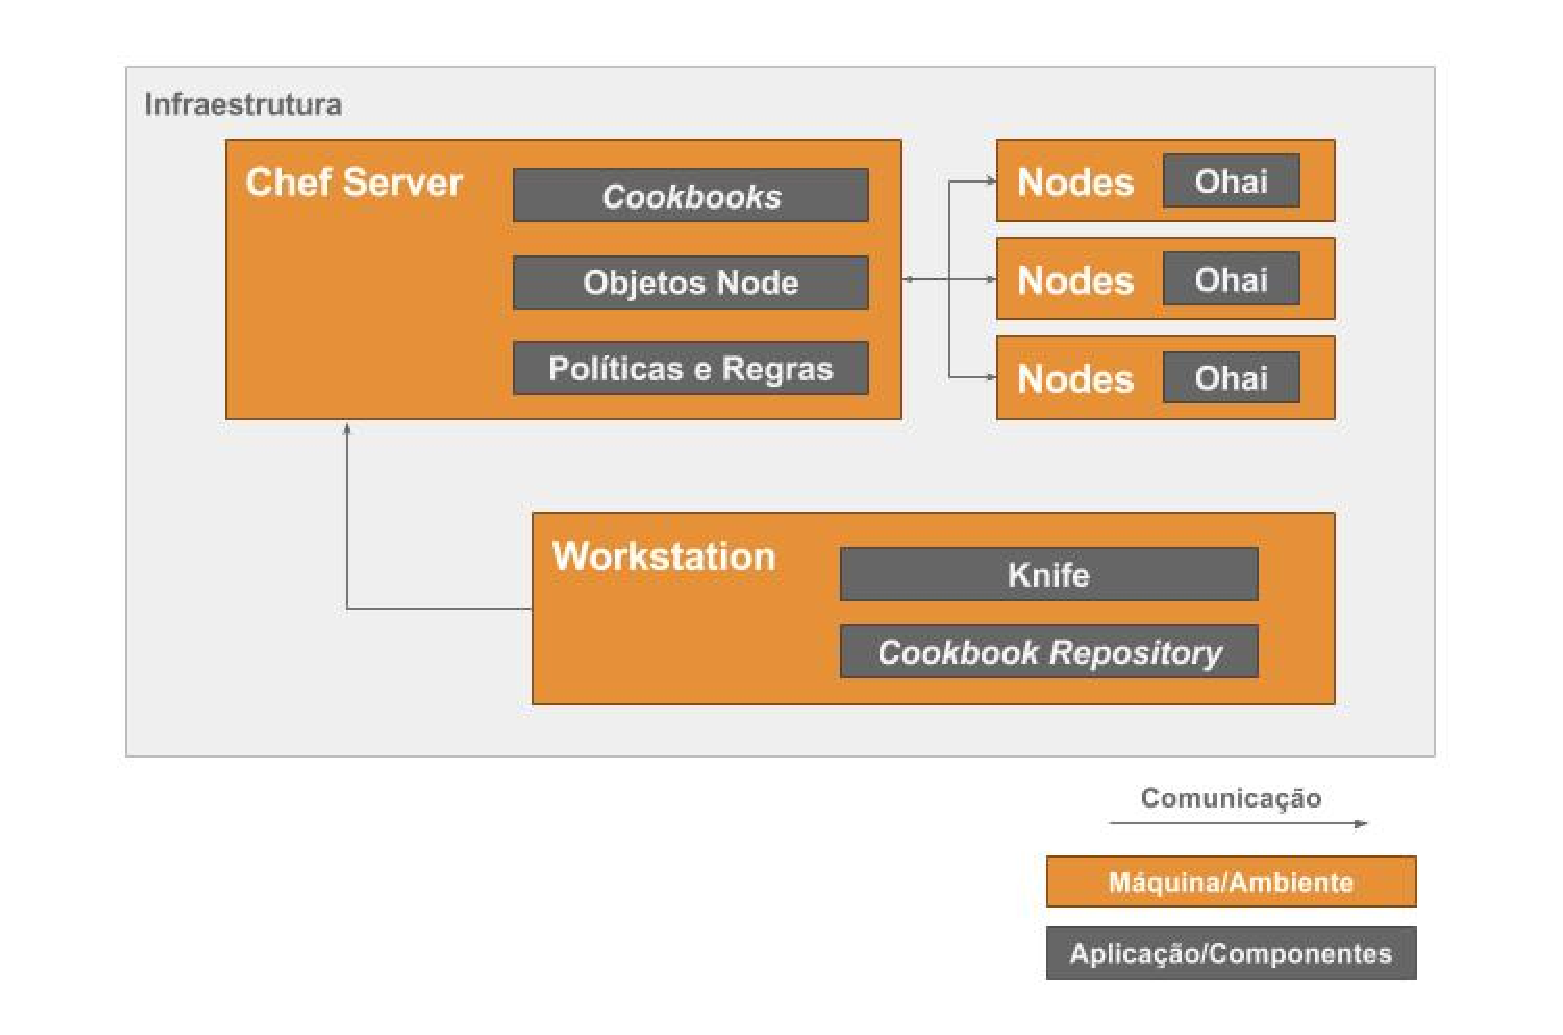
\includegraphics[width=0.9\textwidth]{figuras/chef-comp.eps}
  \caption{Relação entre os componente do Chef}
  \label{fig:chef-comp}
\end{figure}

A ferramenta Chef utiliza os \textit{cookbooks} sendo a unidade básica de configuração do
ambiente. Neles são definidos comandos, arquivos, e outros atributos
para estabelecer o estado desejado para a instalação e configuração
do ambiente alvo \cite{sharma:2015}.

\citeonline{sharma:2015} Classifica os \textit{cookbooks} em três categorias:
\begin{itemize}
  \item \textbf{Aplicação}: contém as configurações de acordo com a instalação de
    uma aplicação. Exemplo PostgreSQL, Apache, Nginx;
  \item \textbf{Biblioteca}: define recursos a serem utilizados por outros \textit{cookbooks}
    (mais detalhes sobre recursos na Seção~\ref{sec:lev-rec} no Capítulo~\ref{chap:lev_es} de levantamento).
    Não é recomendado utilizado diretamente em um node;
  \item \textbf{\textit{Wrapper}}: são \textit{cookbooks} prontos construídos pela comunidade que podem
    ser alterados para que se adequem ao ambiente que será implantado.
\end{itemize}

O componente \textit{chef-client} irá executar as receitas (mais detalhes sobre receitas ou
\textit{recipes} na Seção \ref{sec:lev-rec}) disponíveis nos \textit{cookbooks}
indicados pelo \textit{Chef Server} quando necessário, ou seja, se não houver
nenhuma mudança quanto as configurações do ambiente o \textit{chef-client} não irá
alterar nada, do contrário ele irá aplicar as configurações necessárias~\cite{chefdoc:2016}.





\section{Extração de Configuração}

No processo de automação de uma infraestrutura tem-se a extração das
informações referentes ao sistema. Algumas ferramentas realizam esse
processo como o Ohai~\cite{ohaidoc:2016} e Facter~\cite{facterdoc:2016},
direcionados para o Chef e Puppet, respectivamente. Essas informações
são utilizadas para monitoramento do ambiente controlados pelas ferramentas
de automação.

O método de extração consiste na utilização de outras ferramentas de sistema,
ou seja, a saída da execução de uma ferramenta contém as informações necessárias
a serem extraídas, podendo estar filtradas ou não~\cite{ohaidoc:2016}. O Ohai,
por exemplo, utiliza \textit{plugins} que definem o método de coleta das informações,
a ferramenta de sistema a ser utilizada e o método de filtragem.

Como será visto no Capítulo~\ref{chap:lev_es}, este é o primeiro passo da proposta.
As informações extraídas referem-se às configurações do ambiente. O passo
seguinte é a criação dos \textit{scripts}. Nas pesquisas realizadas, apenas uma ferramenta,
nomeada Blueprint, realiza estes passos.

\subsection{Blueprint}

O Blueprint é uma ferramenta de gerência de configuração que realiza a
engenharia reversa do sistema para extrair, em conjunto a outras ferramentas,
as informações de pacotes, serviços e fontes de instalação de aplicativos
~\cite{blueprint:2016}. O Blueprint foi descontinuado em 2014.

A aplicação é utilizada para criar \textit{scripts} que realizam
a instalação dos pacotes e configurações dos serviços que foram extraídos. Há
também a opção de realizar a conversão desses \textit{scripts} para receitas Chef e módulos
Puppet\footnote{Os módulos Puppet funcionam como receitas Chef, mas são específicos para a ferramenta Puppet.}.
Por esse motivo, o Blueprint é considerado como uma ferramenta concorrente ao Cupper,
pois a sua funcionalidade é semelhante.

A tabela~\ref{tab:cupper-blueprint} mostra uma comparação entre o Cupper e Blueprint.

\begin{table}[H]
  \centering
  \caption{Comparativo entre as ferramentas Cupper e Blueprint}
  \label{tab:cupper-blueprint}
  \begin{tabular}{l|l|l}
    \hline
                                                                       & Cupper                                                                                                   & Blueprint                                                                                     \\ \hline
  \begin{tabular}[c]{@{}l@{}}Informações\\ Extraídas\end{tabular}    & \begin{tabular}[c]{@{}l@{}}Pacotes, serviços,\\ configurações, rede,\\ plataforma, hardware\end{tabular} & \begin{tabular}[c]{@{}l@{}}Pacotes, serviços,\\ configurações\end{tabular}                    \\ \hline
  Saídas                                                             & \textit{Cookbook Chef}                                                                                   & \textit{\begin{tabular}[c]{@{}l@{}}Script Shell, Cookbook\\ Chef, Module Puppet\end{tabular}} \\ \hline
  \begin{tabular}[c]{@{}l@{}}Linguagem de\\ Programação\end{tabular} & \textit{Ruby}                                                                                            & \textit{Python}                                                                               \\ \hline
  \begin{tabular}[c]{@{}l@{}}Gerenciador de\\ Pacotes\end{tabular}   & \begin{tabular}[c]{@{}l@{}}APT/dpkg, Pacman,\\ RubyGem e PIP\end{tabular}                                & \begin{tabular}[c]{@{}l@{}}APT, Yum, RubyGems, easy\_install,\\ PIP, PECL e NPM.\end{tabular} \\ \hline
  \end{tabular}
\end{table}

É considerado como vantagem do Cupper em relação ao seu concorrente:

\begin{itemize}
  \item O Cupper é focado na ferramenta Chef;
  \item O Cupper segue os padrões adotados pelas outras ferramentas do
    Chef;
\end{itemize}

